%=======================================================
% CHAPTER 0: INTRODUCTION
%=======================================================

\begin{frame}[plain]
  \begin{center}\bfseries\centering
    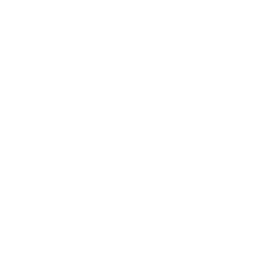
\includegraphics[scale=1]{assets/branding/opa0}
    \vspace{-5.75cm}\\
    {\adjustbox{scale=2.5}{\color{TealDarkCyan}\;I.\;Introduction}}
    \vspace{.25cm}
    \begin{minipage}{.78\textwidth}
      \scriptsize\color{Ink}
      \textbf{Big picture.}\; Lattice cryptography is a story about turning algebraic data into geometric search.\\[.2cm]
      \textbf{Details to watch.}\; basis, determinant, short vectors, dual tests, noise, and modular relations.
    \end{minipage}
    {\ }\vspace{2.1cm}\\
    \bigskip
  \end{center}
\end{frame}

\begin{frame}{\textbf{I. Introduction}}{Discrete Geometry}\small
\textcolor{TealDarkCyan}{\textbf{A lattice is a collection of periodic points.}}
\begin{itemize}
	\item It is discrete, but it fills all directions of a vector space.
	\item It has algebraic data: a basis and integer coefficients.
	\item It has geometric data: length, angle, volume, and distance.
\end{itemize}
\bigskip
\begin{center}
\begin{tikzpicture}[scale=.6]
\clip (-3.2,-2.6) rectangle (3.4,3.0);
\foreach \i in {-4,...,4}{
	\foreach \j in {-4,...,4}{
		\coordinate (p) at ({\i+0.42*\j},{0.72*\j});
		\node[lattice point] at (p) {};
	}
}
\draw[fill=AccentCyan!12,draw=AccentCyan!70,line width=.8pt]
(0,0) -- (1,0) -- (1.42,.72) -- (.42,.72) -- cycle;
\draw[basis vector, magenta] (0,0) -- (1,0) node[right] {$b_1$};
\draw[basis vector, magenta] (0,0) -- (.42,.72) node[above] {$b_2$};
\node[caption text,align=center] at (0,-1.25) {one basis\\ one fundamental cell};
\end{tikzpicture}
\end{center}
\bigskip
\textbf{\color{red}Question.}\; How hard is it to find the closest or shortest lattice vector?
\end{frame}

\begin{frame}{\textbf{I. Introduction}}{Build-up: From Lattices to Cryptography}
\small
\begin{columns}[T,onlytextwidth]
\begin{column}{.46\textwidth}
\textcolor{TealDarkCyan}{\textbf{Big picture}}
\begin{itemize}
  \item Lattices give a bridge from integer algebra to Euclidean geometry.
  \item Hard problems ask for hidden short or nearby structure.
  \item Cryptography publishes the algebra and hides the geometric witness.
\end{itemize}
\end{column}
\begin{column}{.50\textwidth}
\textcolor{TealDarkCyan}{\textbf{Details that will recur}}
\begin{itemize}
  \item \textbf{Shortness:} SIS and Module-SIS ask for short kernel relations.
  \item \textbf{Noise:} LWE, Ring-LWE, and Module-LWE blur exact equations.
  \item \textbf{Rounding:} LWR hides low-order information without sampled error.
\end{itemize}
\end{column}
\end{columns}
\begin{center}
\begin{tikzpicture}[node distance=.72cm,scale=.86,transform shape]
  \node[process] (basis) {basis\\$\mat B\Z^n$};
  \node[process blue,right=of basis] (geom) {geometry\\$\lambda_i,\det,\Ldual$};
  \node[process amber,right=of geom] (hard) {hard tasks\\SVP/CVP/SIS/LWE};
  \node[process red,right=of hard] (crypto) {crypto\\public algebra};
  \draw[flow] (basis) -- (geom);
  \draw[flow blue] (geom) -- (hard);
  \draw[flow amber] (hard) -- (crypto);
\end{tikzpicture}
\end{center}
\textbf{Teaching rule.}\; On each slide, separate the local calculation from the global question:
what public object is given, what hidden witness exists, and why finding it is hard.
\end{frame}

\begin{frame}{\textbf{I. Introduction}}{Why Lattices Matter: Geometry of Numbers}
\scriptsize
\begin{columns}[T,onlytextwidth]
\begin{column}{.60\textwidth}
\defbox[Q. What concrete problem does it solve?]{
\textbf{Example.}\;
In $\Z^2$, Minkowski's theorem says that any centrally symmetric convex region with area $>4$ contains a nonzero integer point.
The statement is geometric, but the conclusion is arithmetic: an integer solution must exist.

\textbf{What it reveals.}\;
A lattice point is not found by solving equations one-by-one; it is forced by volume.
For a general lattice, the threshold is $2^n\det(\Lat)$.

\textbf{Why important.}\;
This is the basic move of lattice theory: prove the existence of number-theoretic objects by showing that Euclidean space has no room to avoid them.}
\end{column}
\begin{column}{.36\textwidth}
\begin{center}
\begin{tikzpicture}[scale=.58]
  \draw[thin lattice line] (-2.6,-2.1) grid[step=.7] (2.6,2.1);
  \foreach \x in {-3,...,3}{
    \foreach \y in {-2,...,2}{
      \node[lattice point] at (.7*\x,.7*\y) {};
    }
  }
  \draw[fill=AccentCyan!13,draw=AccentCyan!80,line width=1pt]
    (0,0) ellipse (1.72 and 1.08);
  \node[circle,draw=ErrorRed,fill=ErrorRed!25,inner sep=2.2pt] at (.7,0) {};
  \node[tiny label,ErrorRed!85!black] at (1.45,.35) {forced point};
  \draw[flow red] (1.25,.25) -- (.75,.03);
  \node[caption text,align=center] at (0,-1.75)
    {$\vol(K)>4\det(\Z^2)$\\$\Rightarrow K\cap\Z^2\ne\{0\}$};
\end{tikzpicture}
\end{center}
\end{column}
\end{columns}
\end{frame}

\begin{frame}{\textbf{I. Introduction}}{Why Lattices Matter: Quadratic Forms}
\scriptsize
\begin{columns}[T,onlytextwidth]
\begin{column}{.58\textwidth}
\defbox[Q. What is the example?]{
\textbf{Example.}\;
The hexagonal lattice has basis
\[
  b_1=(1,0),\qquad b_2=(1/2,\sqrt{3}/2).
\]
For $z=(x,y)\in\Z^2$,
\[
  \norm{x b_1+y b_2}^2=x^2+xy+y^2.
\]

\textbf{What it reveals.}\;
The shortest nonzero vectors are exactly the integer solutions of
\[
  x^2+xy+y^2=1.
\]
There are six of them, which is why each disk in the hexagonal packing touches six neighbors.

\textbf{Why important.}\;
A quadratic form is not just algebraic notation; it is the length function of a lattice written in integer coordinates.}
\end{column}
\begin{column}{.38\textwidth}
\begin{center}
\begin{tikzpicture}[scale=.70]
  \clip (-2.15,-2.35) rectangle (2.25,2.05);
  \foreach \i in {-3,...,3}{
    \foreach \j in {-3,...,3}{
      \coordinate (p) at ({\i+.5*\j},{.866*\j});
      \node[lattice point] at (p) {};
    }
  }
  \draw[ErrorRed!35,line width=.8pt] (0,0) circle (1);
  \foreach \p in {(1,0),(-1,0),(.5,.866),(-.5,.866),(.5,-.866),(-.5,-.866)}{
    \draw[short vector] (0,0) -- \p;
  }
  \draw[basis vector] (0,0) -- (1,0) node[below] {$b_1$};
  \draw[basis vector] (0,0) -- (.5,.866) node[above right] {$b_2$};
  \node[tiny label,align=center,text width=3.0cm] at (0,-1.68)
    {$x^2+xy+y^2=1$\\six shortest vectors};
\end{tikzpicture}
\end{center}
\end{column}
\end{columns}
\end{frame}

\begin{frame}{\textbf{I. Introduction}}{Why Lattices Matter: Diophantine Approximation}
\scriptsize
\begin{columns}[T,onlytextwidth]
\begin{column}{.58\textwidth}
\defbox[Q. How does approximation become a lattice problem?]{
\textbf{Example.}\;
To approximate $\pi$, look for integers $p,q$ with $|p-q\pi|$ tiny.
The famous approximation
\[
  \frac{355}{113}\approx \pi
\]
means that the integer vector $(p,q)=(355,113)$ makes the linear form $p-q\pi$ unusually small.

\textbf{Lattice viewpoint.}\;
For a scale $N$, vectors of the form
\[
  (p-q\pi,\ q/N)
\]
balance two demands: small error and not-too-large denominator.

\textbf{Why important.}\;
Lattices explain why good approximations are short vectors: the numerator, denominator, and error become one geometric object.}
\end{column}
\begin{column}{.38\textwidth}
\begin{center}
\begin{tikzpicture}[x=1cm,y=1cm,scale=.78]
  \draw[->,Ink!75] (-2.0,0) -- (2.0,0) node[right,tiny label] {$p-q\pi$};
  \draw[->,Ink!75] (0,-.2) -- (0,2.55) node[above,tiny label] {$q/N$};
  \draw[Grid,line width=.4pt] (-1.7,.4) -- (1.8,2.15);
  \draw[Grid,line width=.4pt] (-1.5,1.7) -- (1.5,.2);
  \node[circle,fill=Ink!55,inner sep=1.5pt] at (.95,.92) {};
  \node[tiny label,Ink!70] at (1.28,.8) {ordinary};
  \draw[short vector] (0,0) -- (.08,1.65)
    node[above right,tiny label,ErrorRed!85!black] {$355/113$};
  \draw[dashed,ErrorRed!70] (.08,0) -- (.08,1.65);
  \draw[<->,ErrorRed!70,line width=.6pt] (0,-.11) -- (.08,-.11);
  \node[tiny label,ErrorRed!85!black,align=center] at (.85,.22)
    {tiny\\error};
  \node[caption text,align=center] at (0,-.55)
    {short vector balances\\error and denominator};
\end{tikzpicture}
\end{center}
\end{column}
\end{columns}
\end{frame}

\begin{frame}{\textbf{I. Introduction}}{Why Lattices Matter: Sphere Packing}
\scriptsize
\begin{columns}[T,onlytextwidth]
\begin{column}{.56\textwidth}
\defbox[Q. What is the concrete packing example?]{
\textbf{Example.}\;
In the square lattice $\Z^2$, unit spacing gives disk density
\[
  \Delta(\Z^2)=\frac{\pi(1/2)^2}{1}=\frac{\pi}{4}\approx .785.
\]
In the hexagonal lattice, the same nearest-neighbor distance gives
\[
  \Delta=\frac{\pi}{\sqrt{12}}\approx .907.
\]

\textbf{What it reveals.}\;
The key quantities are the shortest vector length $\lambda_1(\Lat)$ and the cell area $\det(\Lat)$.

\textbf{Why important.}\;
The best two-dimensional packing is not discovered by drawing many circles; it is explained by the geometry of one lattice cell and its shortest vectors.}
\end{column}
\begin{column}{.40\textwidth}
\begin{center}
\begin{tikzpicture}[scale=.55]
  \begin{scope}[shift={(-2.0,0)}]
    \foreach \x in {-1,0,1}{
      \foreach \y in {-1,0,1}{
        \draw[fill=BlueCode!9,draw=BlueCode!35] (\x,\y) circle (.5);
        \node[lattice point] at (\x,\y) {};
      }
    }
    \draw[draw=BlueCode!80,line width=.8pt] (-.5,-.5) rectangle (.5,.5);
    \node[caption text,align=center] at (0,-1.85) {square\\$\pi/4$};
  \end{scope}
  \begin{scope}[shift={(2.25,0)}]
    \foreach \i in {-1,0,1}{
      \foreach \j in {-1,0,1}{
        \coordinate (p) at ({\i+.5*\j},{.866*\j});
        \draw[fill=AccentCyan!9,draw=AccentCyan!35] (p) circle (.5);
        \node[lattice point] at (p) {};
      }
    }
    \draw[draw=AccentCyan!85,line width=.8pt]
      (0,0) -- (1,0) -- (1.5,.866) -- (.5,.866) -- cycle;
    \node[caption text,align=center] at (.45,-1.85) {hexagonal\\$\pi/\sqrt{12}$};
  \end{scope}
  \node[caption text,align=center,text width=3.6cm] at (.18,2.0)
    {$\lambda_1$: disk radius\\$\det(\Lat)$: cell area};
\end{tikzpicture}
\end{center}
\end{column}
\end{columns}
\end{frame}

\begin{frame}{\textbf{I. Introduction}}{Why Lattices Matter: Integer Programming}
\scriptsize
\begin{columns}[T,onlytextwidth]
\begin{column}{.58\textwidth}
\defbox[Q. Where does lattice geometry enter optimization?]{
\textbf{Example.}\;
An integer program asks for a point in
\[
  P\cap\Z^n,
\]
where $P$ is a polytope. Its linear relaxation searches $P\cap\R^n$ instead.
A fractional optimum may sit near the middle of a face, while every nearby integer point violates a constraint.

\textbf{What it reveals.}\;
Rounding is a geometric question: how is the real feasible region positioned relative to the lattice $\Z^n$?
If $P$ is thin in some integer direction, that direction is the useful branch or cut.

\textbf{Why important.}\;
Lattice width, flatness, and rounding explain why continuous optimization is only the beginning of integer optimization.}
\end{column}
\begin{column}{.38\textwidth}
\begin{center}
\begin{tikzpicture}[scale=.66]
  \draw[thin lattice line] (-.4,-.4) grid[step=.65] (4.15,3.5);
  \foreach \x in {0,...,6}{
    \foreach \y in {0,...,5}{
      \node[circle,fill=Ink!55,inner sep=1.25pt] at (.65*\x,.65*\y) {};
    }
  }
  \draw[fill=AccentCyan!12,draw=AccentCyan!85,line width=1pt]
    (.42,.35) -- (3.65,.95) -- (2.25,2.72) -- (.72,2.05) -- cycle;
  \node[circle,fill=ErrorRed,inner sep=2.2pt] at (3.25,1.08) {};
  \node[tiny label,ErrorRed!85!black,align=center] at (3.12,1.48) {fractional\\optimum};
  \draw[flow red] (3.25,1.08) -- (2.6,1.3);
  \draw[ErrorRed!80,dashed,line width=.8pt] (.25,1.72) -- (3.9,2.4);
  \node[tiny label,ErrorRed!85!black,align=center] at (2.9,2.75) {cut / thin\\direction};
  \node[caption text,align=center,text width=3.45cm] at (1.8,-.8)
    {$P\cap\R^n$ is easy;\\$P\cap\Z^n$ depends on the grid};
\end{tikzpicture}
\end{center}
\end{column}
\end{columns}
\end{frame}

\begin{frame}{\textbf{I. Introduction}}{Why Lattices Matter: LLL Reduction}
\scriptsize
\begin{columns}[T,onlytextwidth]
\begin{column}{.58\textwidth}
\defbox[Q. What does LLL actually uncover?]{
\textbf{Example.}\;
The vectors
\[
  c_1=(1001,1000),\qquad c_2=(1000,999)
\]
form a basis of $\Z^2$ because $\det[c_1\ c_2]=-1$.
Both basis vectors have length about $1414$, but
\[
  c_1-c_2=(1,1)
\]
is very short.

\textbf{What it reveals.}\;
A basis can hide the geometry of its own lattice.
LLL performs integer column operations to expose shorter, more orthogonal directions.

\textbf{Why important.}\;
Many attacks and algorithms begin by asking: is the secret simply hidden by a bad basis? LLL is the first systematic test.}
\end{column}
\begin{column}{.38\textwidth}
\begin{center}
\begin{tikzpicture}[scale=.74]
  \draw[thin lattice line] (-.2,-.2) grid[step=.55] (3.4,3.1);
  \foreach \x in {0,...,6}{
    \foreach \y in {0,...,5}{
      \node[circle,fill=Ink!45,inner sep=1pt] at (.55*\x,.55*\y) {};
    }
  }
  \coordinate (O) at (0,0);
  \coordinate (cOne) at (2.75,2.6);
  \coordinate (cTwo) at (2.48,2.33);
  \draw[basis vector] (O) -- (cOne) node[above right] {$c_1$};
  \draw[basis vector] (O) -- (cTwo) node[below right] {$c_2$};
  \draw[short vector] (cTwo) -- (cOne) node[midway,right,tiny label] {$c_1-c_2$};
  \draw[short vector] (O) -- (.55,.55) node[above left,tiny label] {short};
  \node[caption text,align=center] at (1.62,-.55)
    {long nearly-parallel basis\\hides a short difference};
\end{tikzpicture}
\end{center}
\end{column}
\end{columns}
\end{frame}

\begin{frame}{\textbf{I. Introduction}}{Why Lattices Matter: Post-Quantum Cryptography}
\scriptsize
\begin{columns}[T,onlytextwidth]
\begin{column}{.58\textwidth}
\defbox[Q. What is the concrete cryptographic shape?]{
\textbf{Example.}\;
In LWE, the public data has the form
\[
  b=\mat A s+e\pmod q,
\]
where $s$ is secret and $e$ is small noise.
Without $e$, this is ordinary linear algebra modulo $q$.
With $e$, it becomes a noisy decoding problem.

\textbf{Lattice viewpoint.}\;
After lifting modulo $q$ to integers, $b$ is close to a structured $q$-ary lattice point, but the small error hides which one.

\textbf{Why important.}\;
Known quantum algorithms are excellent at exact algebraic structure; lattice cryptography deliberately adds controlled noise and shortness constraints.}
\end{column}
\begin{column}{.38\textwidth}
\begin{center}
\begin{tikzpicture}[scale=.64]
  \clip (-2.25,-2.15) rectangle (2.65,2.25);
  \foreach \i in {-3,...,3}{
    \foreach \j in {-3,...,3}{
      \coordinate (p) at ({\i+.45*\j},{.72*\j});
      \node[lattice point] at (p) {};
    }
  }
  \coordinate (As) at (.9,.72);
  \coordinate (b) at (1.18,.98);
  \draw[ErrorRed!35,fill=ErrorRed!7] (As) circle (.42);
  \node[circle,fill=BlueCode,inner sep=2pt,label={[tiny label]below:$\mat A s$}] at (As) {};
  \node[circle,fill=ErrorRed,inner sep=2pt] at (b) {};
  \node[tiny label,ErrorRed!85!black] at (1.55,1.12) {$b$};
  \draw[flow red] (As) -- node[midway,above,tiny label] {$e$} (b);
  \node[tiny label,align=center,text width=3.25cm,fill=white,inner sep=1.5pt] at (.1,-1.05)
    {without noise: linear algebra\\with noise: decoding};
\end{tikzpicture}
\end{center}
\end{column}
\end{columns}
\end{frame}

\begin{frame}{\textbf{I. Introduction}}{Why Lattices Matter: Worst-case to Average-case}
\scriptsize
\begin{columns}[T,onlytextwidth]
\begin{column}{.58\textwidth}
\defbox[Q. Why is this stronger than a random puzzle assumption?]{
\textbf{Example.}\;
A cryptographic public key should look random, so an attacker sees an average-case LWE or SIS instance, not a handcrafted worst-case lattice.

\textbf{Reduction idea.}\;
For suitable parameters, an algorithm that solves random LWE/SIS instances would imply algorithms for approximate GapSVP/SIVP on arbitrary lattices.
The random instance is tied back to the worst lattice geometry.

\textbf{Why important.}\;
This is rare in cryptography: the security evidence for random public instances is connected to broad worst-case mathematical hardness, not only to failed attack attempts.}
\end{column}
\begin{column}{.38\textwidth}
\begin{center}
\begin{tikzpicture}[node distance=.55cm,scale=.78,transform shape]
  \node[process red,minimum width=2.25cm] (worst) {arbitrary\\worst-case\\lattice};
  \node[process blue,below=of worst,minimum width=2.25cm] (reduce) {randomizing\\reduction};
  \node[process amber,below=of reduce,minimum width=2.25cm] (avg) {random\\LWE/SIS\\instance};
  \node[process,below=of avg,minimum width=2.25cm] (break) {average-case\\solver};
  \draw[flow red] (worst) -- (reduce);
  \draw[flow blue] (reduce) -- (avg);
  \draw[flow amber] (avg) -- (break);
  \draw[flow,bend left=42] (break.east) to node[right,tiny label,align=center] {would solve\\worst case} (worst.east);
\end{tikzpicture}
\end{center}
\end{column}
\end{columns}
\vfill
\textbf{Note.}\; The same object can be easy to describe by a basis and difficult to understand geometrically.
\end{frame}

\begin{frame}{\textbf{I. Introduction}}{The Dictionary}
\small
\begin{center}
\renewcommand{\arraystretch}{1.28}
\begin{tabular}{>{\bfseries}p{.28\textwidth}p{.62\textwidth}}
\toprule
Algebra & Geometry \\
\midrule
Basis matrix $\mat B$ & Skew coordinate grid in $\R^m$ \\
Integer vector $\vect z\in\Z^n$ & Lattice point $\mat B\vect z$ \\
Unimodular change $\mat U\in\GL_n(\Z)$ & Same lattice, different basis \\
$|\det \mat B|$ & Volume of a fundamental cell \\
Dual basis $\mat B^{-T}$ & Linear tests taking integer values \\
\bottomrule
\end{tabular}
\end{center}
\vfill
\textbf{\color{red}Warning.}\; A good coordinate system is not automatic. A bad basis can hide very short vectors.
\end{frame}

\begin{frame}{\textbf{I. Introduction}}{Roadmap}
\small
\begin{enumerate}
  \item Define lattices, bases, determinant, and the dual lattice.
  \item Use geometry of numbers to prove that short vectors must exist.
  \item State the main computational lattice problems.
  \item Explain why SIS, LWE, Ring-LWE, Module-LWE, LWR, and Module-SIS are lattice problems in disguise.
\end{enumerate}
\bigskip
\begin{center}
\begin{tikzpicture}[node distance=.7cm]
  \node[process] (basis) {basis};
  \node[process blue, right=1.1cm of basis] (geom) {geometry};
  \node[process amber, right=1.1cm of geom] (hard) {hard problems};
  \node[process red, right=1.1cm of hard] (crypto) {LWE/SIS\\families};
  \draw[flow] (basis) -- (geom);
  \draw[flow blue] (geom) -- (hard);
  \draw[flow amber] (hard) -- (crypto);
\end{tikzpicture}
\end{center}
\end{frame}
